\section{Topology Comparison: Serial, Hybrid, and Parallel}
\label{sec:topology}

Having established in \cref{sec:architecture-trade} that a constellation of many
inexpensive relay satellites is the preferred architecture, the next design decision
is how to \emph{arrange} those satellites. The topology determines how data flows
from Earth to Mars: how many independent paths exist, which link is the bottleneck,
and how the constellation responds to individual satellite failures. We evaluate three
candidate topologies---serial, hybrid, and parallel---against four criteria:
aggregate throughput scaling, redundancy, failure tolerance, and hardware complexity
per satellite. \Cref{fig:topology-schematic} illustrates the three topologies
schematically.

\begin{figure}[t]
  \centering
  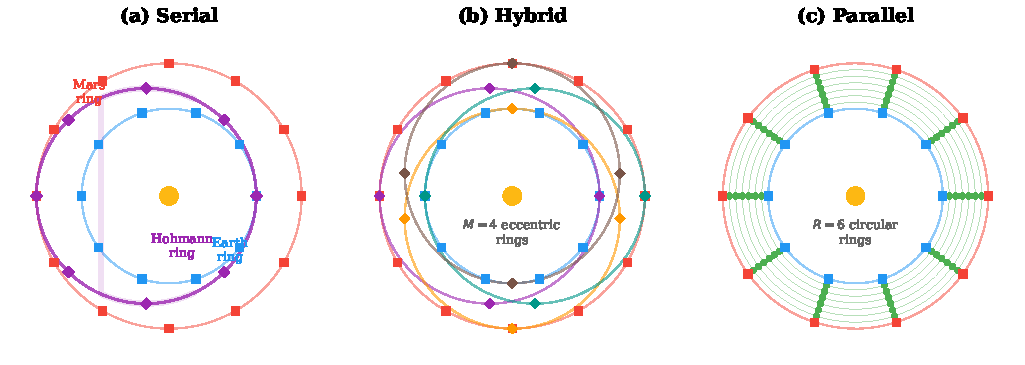
\includegraphics[width=\textwidth]{figures/topology-schematic.pdf}
  \caption{Schematic comparison of the three relay topologies (top-down
    heliocentric view). \textbf{(a)}~Serial: a single transfer-orbit ring
    connects the Earth and Mars circular rings at perihelion and aphelion.
    \textbf{(b)}~Hybrid: $M$ transfer-orbit rings with staggered arguments of
    perihelion improve coverage. \textbf{(c)}~Parallel: $R$ concentric
    rings create $N$ independent radial routes.}
  \label{fig:topology-schematic}
\end{figure}


\subsection{Serial Relay (Single Transfer Orbit)}
\label{sec:topo-serial}

The most intuitive relay topology uses three orbital rings. A circular
\emph{Earth ring} of $N_E$ satellites orbits at heliocentric radius $\rE$. A
circular \emph{Mars ring} of $N_M$ satellites orbits at $\rM$. Between them, a
single \emph{transfer ring} of $N_H$ satellites follows an elliptical
Hohmann-like orbit whose perihelion coincides with $\rE$ and whose aphelion
coincides with $\rM$. Data flows in series: ground stations hand off to the Earth
ring, the Earth ring relays to the transfer ring near perihelion, the transfer
ring relays to the Mars ring near aphelion, and the Mars ring delivers to the
surface.

Each satellite on the Earth and Mars rings carries two laser terminals
(circumferential, to maintain the ring) plus one inter-ring terminal pointing
toward the transfer ring. Each transfer-ring satellite carries two circumferential
terminals plus two inter-ring terminals (one Earth-facing, one Mars-facing),
for a total of four.

The bottleneck is the inter-ring link. At perihelion, transfer-ring satellites are
co-orbital with the Earth ring, and the link distance is set by the angular
separation between the nearest satellites on each ring---of order $\pi \rE / N_E$
for the Earth ring. At aphelion, the same applies at Mars: the link distance is of
order $\pi \rM / N_M$. Between these extremes, transfer-ring satellites spend the
majority of their orbital period at intermediate heliocentric distances where they
are far from both planetary rings. During cruise, the link to the nearest planetary
ring spans a distance of order $\Dem / 2 \approx 39\;\text{Mkm}$, and the
inverse-square law reduces per-link capacity to
%
\begin{equation}\label{eq:hohmann-cruise}
  C_{\text{cruise}} \;\sim\; \frac{K}{(\Dem/2)^2}
  \;=\; \frac{4K}{\Dem^2}
\end{equation}
%
For the baseline parameters ($K = 9 \times 10^{8}\Gbps\cdot\text{km}^2$,
$\Dem = 78 \times 10^{6}\km$), this gives approximately $0.6\;\text{kbps}$---far
below any useful threshold. The transfer ring is only effective when its satellites
are near perihelion or aphelion; the rest of the orbit is a dead zone.

Because the interplanetary segment passes through a single transfer ring, the
topology has only one data path between Earth and Mars at any given time. This
creates a single point of failure: the loss of the active transfer-ring relay
severs the link entirely. The Earth and Mars rings provide local redundancy (a
failed satellite on either circular ring can be bypassed via its neighbours), but
this is irrelevant if the interplanetary hop is broken.

Throughput does not scale well with constellation size. Adding satellites to the
Earth or Mars rings improves local connectivity but does nothing for the
interplanetary bottleneck. Adding satellites to the transfer ring increases the
number of potential relay nodes near perihelion and aphelion, but only one is
active at a time (the one closest to the handoff point), so throughput remains
limited to a single inter-ring link.


\subsection{Hybrid Relay (Multiple Transfer Orbits)}
\label{sec:topo-hybrid}

The hybrid topology retains the Earth and Mars circular rings of the serial
configuration but replaces the single transfer ring with $M$ transfer rings, each
on its own Hohmann-like orbit. All $M$ orbits share the same semi-major axis and
eccentricity (perihelion at $\rE$, aphelion at $\rM$) but have their arguments
of perihelion equally spaced at intervals of $360^\circ/M$. This angular staggering
ensures that, at any instant, the $M$ transfer rings are distributed around the
Sun at different phases of their orbits, so that at least some satellites are
always near one of the two planetary rings.

The motivation is to address the dead-zone problem of the serial topology.
With $M$ transfer rings, the probability that \emph{some} transfer satellite is
near perihelion or aphelion at any given time increases with $M$. For large
enough $M$, the constellation can maintain near-continuous handoff between the
Earth ring and whichever transfer ring is currently closest, and likewise between
the Mars ring and its nearest transfer neighbour.

However, the fundamental throughput bottleneck remains. Each transfer ring still
traverses the full Earth--Mars gap, and a satellite on any such ring spends the
majority of its orbital period at intermediate heliocentric distances where the
link to either planetary ring spans tens of millions of kilometres. The
inverse-square penalty during cruise (\cref{eq:hohmann-cruise}) applies
identically to every transfer ring. Staggering the arguments of perihelion
improves \emph{availability}---the fraction of time that at least one usable
relay exists---but does not improve the \emph{throughput} of any individual relay
during cruise.

The hybrid topology does gain a measure of redundancy over the serial
configuration. With $M$ transfer rings, the loss of one ring still leaves $M - 1$
alternative interplanetary paths. But each path independently suffers the same
cruise-phase throughput floor, so the aggregate capacity scales at best linearly
with $M$---and only during the favourable orbital phases when a transfer
satellite is near a planetary ring. During cruise, additional transfer rings add
satellites that contribute negligible throughput.

Hardware complexity also increases. Each transfer-ring satellite requires four
laser terminals (two circumferential, one Earth-facing, one Mars-facing), and the
pointing geometry changes continuously along the eccentric orbit. Satellites on
the Earth and Mars rings need additional terminals to maintain links with
whichever transfer ring is currently nearby. The total terminal count per
satellite is 3--4, compared with 2 for the parallel topology.

\Cref{fig:throughput-vs-phase} quantifies the dead-zone problem. For a single
transfer ring ($M = 1$), the best available inter-ring link capacity drops by over
eight orders of magnitude between the perihelion/aphelion peaks and the mid-orbit
trough. Adding transfer rings ($M = 3, 6$) raises the envelope by introducing
peaks at intermediate phases, but the capacity between peaks remains far below the
constant throughput achievable with the parallel topology.

\begin{figure}[t]
  \centering
  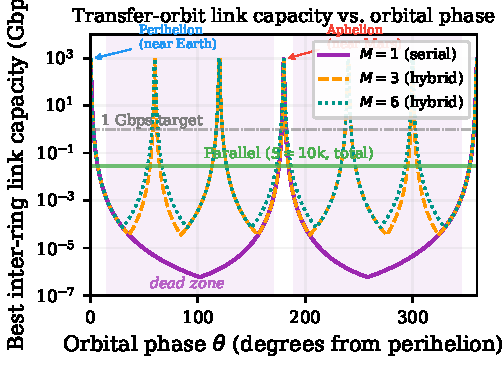
\includegraphics[width=0.75\columnwidth]{figures/throughput-vs-phase.pdf}
  \caption{Best available inter-ring link capacity as a function of orbital
    phase for the serial ($M = 1$) and hybrid ($M = 3, 6$) topologies.
    The horizontal green line shows the total throughput of a parallel
    constellation with $S = 10{,}000$ satellites at optimal ring allocation.
    Baseline parameters: $f = 1$, $K = 9 \times 10^{8}\Gbps\cdot\text{km}^2$.}
  \label{fig:throughput-vs-phase}
\end{figure}


\subsection{Parallel Relay (Concentric Orbits)}
\label{sec:topo-parallel}

The parallel topology distributes the $S$ satellites across $R$ concentric
heliocentric orbits (``rings'') between Earth and Mars. Each ring
contains $N = S/R$ satellites evenly spaced around its circumference. Every
satellite carries exactly two laser terminals: one pointing radially inward to
the nearest satellite on the adjacent inner ring, and one pointing radially outward
to the nearest satellite on the adjacent outer ring. There are no circumferential
(intra-ring) links.

This arrangement creates $N$ independent parallel routes from Earth to Mars, each
consisting of a radial chain of $R$ inter-ring hops. The throughput of each route
is limited by its bottleneck link (the outermost inter-ring gap, as derived in
\cref{sec:worst-case}), and the total constellation throughput is the sum over all
$N$ routes:
%
\begin{equation}\label{eq:parallel-throughput}
  T_{\text{parallel}} \;=\; N \cdot \frac{K}{d_{\max}^2}
\end{equation}
%
As shown in \cref{sec:scaling-law}, optimising the distribution between rings and
routes yields $T_{\text{opt}} \propto S^{3/2}$. This super-linear scaling is the
parallel topology's defining advantage: every satellite added improves both the
per-route capacity (by shortening inter-ring distances) and the aggregate capacity
(by adding routes).

Redundancy is intrinsic. The loss of a single satellite removes one route from one
ring but leaves all other $N - 1$ routes intact. Throughput degrades gracefully---by
a fraction $1/N$---rather than catastrophically. For a constellation with $N = 100$
routes per ring, losing one satellite reduces total throughput by 1\%.

The hardware requirement is minimal: two laser terminals per satellite, the fewest
of any topology considered. The two terminals point radially (inward and outward),
and each satellite participates in exactly one route. This radial-only pointing
simplifies acquisition and tracking, since adjacent rings are separated by a fixed,
predictable gap.

Scalability follows naturally. Adding satellites to existing rings increases $N$
and therefore the number of parallel routes. Adding new rings between existing
ones increases $R$, shortening inter-ring distances and boosting per-route
capacity. Both operations improve total throughput without requiring any change
to the satellite hardware or link architecture.


\subsection{Topology Comparison}
\label{sec:topo-table}

\Cref{tab:topology-comparison} summarises the key properties of the three
topologies. The serial and hybrid configurations both suffer from the same
fundamental limitation: their interplanetary segments traverse the full Earth--Mars
gap on transfer orbits, spending most of each orbital period at distances where the
inverse-square law renders throughput negligible. The parallel topology avoids this
entirely by breaking the interplanetary gap into many short radial hops on
concentric orbits, achieving both higher throughput and intrinsic redundancy with simpler
hardware.

\begin{table}[t]
  \centering
  \caption{Comparison of relay constellation topologies for $S$ total satellites.}
  \label{tab:topology-comparison}
  \begin{tabular}{@{}lccc@{}}
    \toprule
    \textbf{Property}
      & \textbf{Serial}
      & \textbf{Hybrid}
      & \textbf{Parallel} \\
    \midrule
    Orbital implementation
      & 1 transfer orbit
      & $M$ transfer orbits
      & $R$ concentric orbits \\[3pt]
    Aggregate throughput scaling
      & Single-link limited
      & $\sim\!\!M$ (favourable phase)
      & $S^{3/2}$ ($N$ routes) \\[3pt]
    Parallel data paths
      & 1
      & $\leq M$
      & $N = S/R$ \\[3pt]
    Redundancy
      & Local rings only
      & Local + partial interplanetary
      & Per-route \\[3pt]
    Single-satellite failure
      & Interplanetary outage
      & $1/M$ path loss
      & $1/N$ throughput loss \\[3pt]
    Laser terminals / satellite
      & 3--4
      & 3--4
      & 2 \\[3pt]
    Cruise dead zone
      & Yes (severe)
      & Yes (per ring)
      & None \\[3pt]
    Scalability
      & Add to rings
      & Add transfer orbits
      & Add to rings or add rings \\
    \bottomrule
  \end{tabular}
\end{table}

We adopt the parallel concentric-ring topology for the remainder of this paper.
\Cref{sec:throughput} develops the full throughput model, derives the optimal
allocation between rings and routes, and establishes the $S^{3/2}$ scaling law
that governs the constellation's performance.
